\documentclass[a4paper,11pt,oneside]{report}
% Options: MScThesis, BScThesis, MScProject, BScProject
\usepackage[BScProject]{EPFLreport}
\usepackage{xspace}
\usepackage[T1]{fontenc}
\usepackage{lmodern}
\usepackage{todonotes}
\usepackage{import}
\usepackage{amsmath}

\newcommand{\svg}[1]{\import{./figures/}{#1}}

\title{Applying Approximate Distance Oracles to Internet Routing}
\author{Matteo Pariset}
\supervisor{Cristina Basescu}
\adviser{Prof. Bryan Ford}

\newcommand{\td}[1]{\todo[inline,color=red!40]{TODO: #1}}

\begin{document}
\maketitle

%\maketoc

%%%%%%%%%%%%%%%%%%%%%%
\chapter{Motivation}
%%%%%%%%%%%%%%%%%%%%%%
In order to reach their destinations, IP packets must go through multiple physical devices, across several IP networks. The process of selecting their path is called \emph{routing} and relies on information shared among routers using a \emph{routing protocol}. In the Internet, different protocols are used at different scales. For instance, Open Shortest Path First (OSPF) is typically used for routing packets between sub-networks belonging to the same organization whereas \emph{Border Gateway Protocol} (BGP) is the \textit{de facto} standard for global Internet routing. It operates at the level of \emph{Autonomous Systems} (ASes), administrative entities which are identified by unique \emph{autonomous system numbers} (ASNs).
BGP is a path-vector routing protocol which selects routes based on prefix announcement rules and AS-specific policies.

% A workshop organized by the Internet Architecture Board
\bigskip
Over the years, the impressive evolution of Internet-based services has exposed several of BGP weaknesses, making its scalability a major concern for Internet operators \cite{elmokashfiScalabilityBGPRole2010}. For instance, prefix de-aggregation, resulting from common traffic engineering practices and multi-homing \cite{dReportIABWorkshop}, has provoked a faster-than-linear growth of the Routing Information Base (RIB) size \cite{Potaroo}. Although the RIB is bounded by the address space size\footnote{And the number of adjacent ASes}, the amount of BGP messages needed to react to network changes is not. Prefix de-aggregation ``exposes the core of the network to the dynamic nature of the edges'' \cite{dReportIABWorkshop}, increasing BGP churn, i.e. the number of BGP UPDATE messages sent over the network. A small number of ASes and IP prefixes are responsible for a large fraction of the total UPDATE churn \cite{BGPchurnCore2012}; even worse, part of this information is often superfluous since it is generated by unstable edges \cite{Oliveira_measurementof}.

The exponential growth of BGP routing table (RT), besides being a problem in itself, also entails convergence issues, since UPDATE messages can trigger re-computation of the \emph{forwarding information base} (FIB).

\bigskip
Those issues seem to be inevitable, since Gavoille \textit{et al.} \cite{gavoilleMemoryRequirementRouting1996} showed that BGP, like all stretch-1 universal routing protocols, requires $\Omega(n\log n)$ bits for the RT\footnote{In this chapter, $n$ denotes the number of nodes in the network}. Given that the theoretical upper-bound is also equal to $\mathcal{O}(n\log n)$, BGP achieves the worst possible performances in terms of RT size. It is thus clear that the stretch-1 requirement must be dropped to achieve sustainable, i.e. sub-linear, RT scaling.

The collection of techniques that offer sub-linear growth in RT size is known as \emph{compact routing}.
In this work, we focus on a particular universal compact routing scheme (TZ), by Thorup and Zwick \cite{thorupApproximateDistanceOracles2005}, which ensures:
\begin{itemize}
\item bounded maximum stretch;
\item nearly optimal space requirements;
\item \textbf{constant} query time.
\end{itemize}

Although the worst-case stretch of TZ is far from being acceptable for Internet paths, we know \cite{krioukovCompactRoutingInternet2007} that its average stretch on static, ``Internet-like'' topologies is sufficiently small (close to 1) to make it a viable inter-AS routing algorithm. It is not clear, though, how efficiently TZ would cope with changes in the topology, given that the Internet graph is by no means static. Using general arguments, Afek \textit{et al.} \cite{afekUpperLowerBounds1989} showed that the worst-case communication cost - the number of control messages needed to reach convergence - cannot scale better than $\Omega(n)$.
This result, however, does not provide estimates on the frequency of this worst-case scenario for Internet-like graphs.

\bigskip
Therefore, we are interested in designing and implementing TZ response to topological changes. We limit ourselves to the case of edge failures since other events, like the creation of new edges and the disappearance of an AS, can be treated with methods similar to the ones presented here.

To measure performances of this algorithm, we also build a simulator, capable of executing both BGP and our modified version of TZ on any given topology (loaded from a \texttt{csv} file). It allows to trigger edge deletions, either manually or randomly, and to log multiple metrics. Its source code, written in Go, can be found at \cite{RoutingAlgorithmsSimulator}. To conduct our simulations, we use the entire AS graph rather than smaller synthetic graphs, since those would hardly be representative of the Internet. Additional details on how we derive it, as well as on its structure and evolution over time, can be found in chapter \ref{chap.as-graph}.
In chapter \ref{chap.adapt-tz-internet}, we present a modified version of TZ scheme, better suited to static Internet routing, which is further improved in chapter \ref{chap.dyn_topology} to handle dynamic topologies.

\chapter{The AS graph}
\label{chap.as-graph}

We reconstruct the shape of the Internet at the AS level, using data collected by CAIDA \cite{GraphCAIDA}, available on a monthly basis, starting from December 2015. Inter-AS links, annotated with their types, are inferred using two methodologies, detailed in \cite{luckieRelationshipsCustomerCones2013} and \cite{giotsasInferringMultilateralPeering2013}.

\bigskip
Each link between Autonomous Systems belongs to one of the following categories, which constitute the extremes of a much wider spectrum:
\begin{itemize}
\item \emph{provider-to-customer} \textbf{PC} (resp. \emph{customer-to-provider} \textbf{CP}): it reflects the hierarchical organization of ISPs and generally implies the sale of connectivity by one of the endpoints to the other;
\item \emph{peer-to-peer} \textbf{P2P}: it indicates a bilateral agreement to exchange traffic and routes free of charge.
\end{itemize}
In what follows, we also use the symbols $\searrow$, $\nearrow$ and $\longleftrightarrow$ to indicate PC, CP and P2P links respectively.

\bigskip
Looking at the size of the graph, we observe that the number of ASes kept growing linearly between 2015 and 2020, as already remarked by Dhamdhere and Dovrolis \cite{dhamdhereTenYearsEvolution2008} in 2008. A linear increase can also be seen in the the number of CP links ($+30\%$) (figure \ref{fig.evo-edges-type}). P2P links were, instead, subject to bigger short-term variations, likely determined by the inherent difficulties in discovering them \cite{dhamdhereTenYearsEvolution2008}.

\bigskip
Another meaningful property to inspect is the distribution of the degrees of nodes. That is because, as Krioukov \textit{et al.} \cite{krioukovCompactRoutingInternet2007} noticed, the \emph{scale-free} nature of a graph is crucial to reduce the number of paths with worst-case stretch. In figure \ref{fig.ccdf-as-deg}, we plot the CCDF of AS degrees as measured in 2015, 2019 and 2020. The shift in the Internet contents distribution paradigm, happened over the last decade, has not altered this distribution, which, today as in 2015, follows a power-law. This means that business interactions among ASes can still be accurately described by a preferential attachment process.

The AS degrees distribution, while devoid of radical changes, reveals nonetheless some gradual transformations. In 2020, more nodes have degrees ranging from $100$ to $1000$, compared to 2015. To understand why, in figure \ref{fig.ccdf-as-deg-type} we group nodes according to the most frequent type of incident edges. For example, ``2015 customer'' will be the 2015's degrees distribution, calculated only over ASes predominantly connected to edges of type \textit{customer-provider}. We observe that the shapes of ``customer'' and ``provider'' ASes distributions have not evolved over the last 5 years (brown and blue lines), whereas the nodes with a majority of P2P links tend to have a lower degree in today's Internet.

A possible explanation is offered by conjecturing a progressive flattening of the Internet, as exposed by Wang and Zhang \cite{wangQuantifyingFlatteningInternet2016}, according to which nodes of type ``peer'' are, now, more likely to be middle-sized ASes, instead that tier-1 ISPs.

\begin{figure}[!htb]
\begin{minipage}{0.48\textwidth}
\centering{
\resizebox{85mm}{!}{\svg{ccdf_as_deg.pdf_tex}}
\caption{Evolution of CCDF of AS degrees}
\label{fig.ccdf-as-deg}
}
\end{minipage}\hfill
\begin{minipage}{0.48\textwidth}
\centering{
\resizebox{85mm}{!}{\svg{ccdf-as-deg-maj.pdf_tex}}
\caption{CCDF of AS degrees by type of node}
\label{fig.ccdf-as-deg-type}
}
\end{minipage}\
\end{figure}

\begin{figure}[!htb]
\begin{minipage}{0.48\textwidth}
\centering{
\resizebox{85mm}{!}{\svg{edges_by_type.pdf_tex}}
\caption{Evolution of edges by type, PC links are part of the CP category}
\label{fig.evo-edges-type}
}
\end{minipage}\hfill
\begin{minipage}{0.48\textwidth}
\centering{
\resizebox{85mm}{!}{\svg{edges_types_mut.pdf_tex}}
\caption{Fraction of edges in the stable subgraph that change type}
\label{fig.edges-type-mut}
}
\end{minipage}\
\end{figure}

\bigskip
Since our simulations heavily rely on type annotations, we are also interested in determining the stability of such labels. For this purpose, we consider the sub-graph induced by the nodes that never disappear from our data for the whole period of our analysis (Dec. 2015 to Apr. 2020), which we call \emph{stable graph}. For each month, we then plot (figure \ref{fig.edges-type-mut}) the fraction of edges in the stable graph which change of type. On average only $0.5\%$ of them undergo variations, mostly transitioning from CP to P2P and vice-versa. We believe that these are mostly spurious conversions, since spikes in one kind of transition are shortly followed by higher-than-usual numbers of conversions in the opposite direction.

\chapter{Adapt TZ to the Internet}
\label{chap.adapt-tz-internet}

Before describing our improvements, we briefly introduce the original TZ scheme. Given a graph $G=(V, E)$ and a parameter $k$, the algorithm constructs $k$ sets ($A_i$) of randomly chosen nodes, called \emph{landmarks}. They are such that:
\[
A_0 = V, \qquad 1 \leq i \leq k: A_{i-1} \supset A_i, \qquad A_k = \emptyset
\]

We call the elements in $A_{k-1}$, namely the nodes in the smallest non-empty set, \emph{top-level} landmarks.
Distances to landmarks are used to approximate distances between arbitrary nodes, which are guaranteed to know the distance to, at least, one common landmark. Every node $v$ must maintain two structures:
\begin{itemize}
\item $W(v) = \{W_i(v) \;|\; 0 \leq i \leq k \}$, a collection of distances to \emph{witnesses} $W_i(v)$, which (for each $i$) is the closest landmark in $A_i$ to $v$;
\item $B(v)$, its \emph{bunch}, containing distances to other, well-chosen nodes. In particular, nodes in the bunch are closer to $v$ than $v$ is to some of its witnesses, i.e. $B(v) = \{s \in V \;\vert\; \exists i \leq k \text{ s.t. } \delta(v, s) < \delta(v, W_i)\}$ (where $\delta$ denotes the distance between to vertices)
\end{itemize}

Although the above structures are primarily intended to answer distance queries, they are enough to construct paths between arbitrary pairs of nodes. More on this can be found in \cite{thorupApproximateDistanceOracles2005}.

Henceforth, we adopt the terminology introduced above and set $k=3$.

\section{Landmarks Selection}
\label{sec.landmarks-sel}
TZ authors suggest to select landmarks uniformly at random from nodes in the graph. This strategy, which preserves the generality of the algorithm, becomes sub-optimal when TZ is applied to the AS graph.

Since landmarks roughly serve as middle-points in approximated paths, they should preferably be selected among nodes which play that role in the Internet. We hence exploit our knowledge that the hierarchical organization of ASes favors inverted V-shaped paths, in which traffic climbs the ISP hierarchy to then descend again. Big Internet Service Providers are in fact a good candidate for landmarks, given that they sell Internet connectivity to smaller ISPs.

\bigskip
We then increase the probability that important Autonomous Systems are selected as landmarks. We pay particular attention to the selection of top-level ones (which should be around $|V|^{1-2/k} = 40$), since distances to all of them are known to every node in the graph.
We could define the importance of ASes as the size their customer cones, but we choose to approximate it with the number of incident PC links. We prefer this definition because, although more local, it still efficiently captures the informal notion of ISP importance. It gives $68\%$ agreement over the set of 64 most important ISPs from CAIDA AS rank \cite{CAIDAASRank}.

Our selection strategy, which we call \emph{popularity selection}, assigns to each AS a different selection probability depending on its number of PC links. The most important (according to our definition above) ASes are several orders of magnitude more likely to become landmarks than before but every AS keeps a non-zero probability of being selected. We note that landmark selection strategies do not affect the correctness of the algorithm but can only alter the quality of its path estimates and the size of its structures.

We compare the effects of the selection strategy in figure \ref{fig.landmark-selection-stretch} which contains the distribution of stretch, when popularity (green) and random (red) landmarks selection strategies are used. 

\begin{figure}[!htb]
\begin{minipage}{0.48\textwidth}
\centering{
\resizebox{85mm}{!}{\svg{ladmark-selection-stretch.pdf_tex}}
\caption{Measured stretch depending on landmarks selection strategy, 4000 routes}
\label{fig.landmark-selection-stretch}
}
\end{minipage}\hfill
\begin{minipage}{0.48\textwidth}
\centering{
\resizebox{85mm}{!}{\svg{stretch_with_valley.pdf_tex}}
\caption{Number of routes with valleys (4000 samples), for every stretch interval}
\label{fig.stretch-with-valley}
}
\end{minipage}\
\end{figure}

We generate 4000 paths between random nodes and compare their lengths against the baseline, calculated using BGP. It can be seen that popularity selection performs better, achieving an average stretch of 1.06 compared to 1.17 of random selection.

We also note that some paths have a stretch strictly smaller than 1. This occurs because stretch only depends on hop distance but our baseline paths are not shortest paths, i.e. they are optimal with respect to BGP criteria but non-optimal in terms of stretch. In fact, BGP also filters routes according to link types, preferring for instance a long path constituted of PC edges to a shorter one with P2P ones. To illustrate this, we provide a rather extreme example:

\begin{center}
\begin{tabular}{c|c|c}
&Path between \textbf{AS29827} and \textbf{AS61170}&Hop-length \\
\hline
\textbf{BGP}& $\nearrow {\color{green}\searrow} \searrow \searrow \searrow \searrow \searrow \searrow \searrow \searrow \searrow \searrow$ & 12 \\
\textbf{TZ}& $\nearrow {\color{red}\longleftrightarrow} \searrow$ & 3
\end{tabular}
\end{center}

In the table, BGP does not provide the ``shortest'' path since the second edge of its path (in green, of type PC) is preferred to the second edge of TZ path (in red, of type P2P).

\section{GR compliance}
The example above shows why simple stretch considerations are insufficient to thoroughly assess routing algorithms performances. Traffic on the Internet is subject to complex and AS-dependent economic dynamics which heavy influence the paths it follows. These constraints, together with router-specific software differences, have posed a threat to BGP stability in the past and have prompted the formalization of guidelines which ensure routing algorithm convergence. Here we adopt those formulated by Gao and Rexford \cite{lixingaoStableInternetRouting2001} (we call them GR), which strike a balance between market needs and preconditions for correct Internet routing.

\bigskip
We deem it necessary to understand whether paths generated using TZ scheme comply with GR or similar criteria. 
As a first approximation, we study the presence of \emph{valleys} in path, which signal a specific violation of routes filtering rules. They occur when a node advertises a provider route\footnote{We use provider route as a shorthand for \textit{route whose first hop is a customer-to-provider link}} to some of its providers. This would not be cost effective for that node, and therefore not likely to happen in the real Internet. Even this partial adoption of GR rules is enough to highlight some differences between landmarks selection strategies.
About a third of the paths computed using random selection contain \textit{valleys}, whereas this fraction drops to $11.5\%$ if we use popularity selection. Figure \ref{fig.stretch-with-valley} breaks those figures over unitary stretch intervals. 

\bigskip
Although popularity selection helps to fill the gap between TZ approximations and viable paths, it is unlikely to close it altogether. To guarantee that paths always respect GR requirements it is necessary to directly incorporate them in our routing scheme which, in its basic version, has no knowledge of link types. 

\bigskip
In order to do that, we make TZ apply GR filtering rules, as proposed in \cite{lixingaoStableInternetRouting2001}, when it grows shortest path trees needed to construct both bunches and sets of witnesses.
Distances between nodes are thus obtained using a modified version of Dijkstra's algorithm which, running from a source $d$, relaxes an edge $e$ only if BGP exported the destination $d$ over $e$. We test two variants of filtering rules, which we call GR and GRP. Both of them require node $n$:
\begin{itemize}
\item to export all the routes to its customers;
\item to export customer routes\footnote{Namely the routes with a customer of $n$ as next-hop} to its peers and providers.
\end{itemize}
The only difference between the two variants is that, under GRP, $n$ can also announce peer routes to its peers, i.e. it can provide transit services to its peers. This assumption is interesting since it captures a different use of P2P links, which could be realistic under the hypothesis of a flattening Internet.

\bigskip
To restore the correctness of the modified TZ, some adjustments become necessary. In particular, since distances - calculated using GR/P filtering - do not satisfy the triangle inequality, nodes in bunches are no longer guaranteed to induce a spanning tree. For each node $n$, we hence restore this invariant by completing its bunch $B(n)$ with all the nodes on the shortest path between $n$ and every $a \in B(n)$.

Another issue concerns nodes that become unreachable, i.e. those which filtering rules make invisible to some other nodes. They are a small fraction of ASes ($0.5\%$), probably resulting from spurious noise in type annotations described in chapter \ref{chap.as-graph}. In those cases, we allow paths to violate route filtering rules, so that every destination is reachable.
In all the other cases, this version of TZ scheme ensures that paths never contain valleys.

\chapter{TZ on dynamic topologies}
\label{chap.dyn_topology}

We now examine what happens when a link between ASes becomes unavailable, following either a technical failure or a deliberate action. This translates into the disappearance of the corresponding edge from our AS graph. We suppose that, after a certain time delay, both endpoints become aware of the failure and we analyze the consequences of this circumstance on (our version of) TZ structures.

\bigskip
It is possible that the endpoints (and other nodes) relied on the missing edge to reach some of their witnesses or some destinations in their bunches. If they simply dropped these destinations, some routing processes could fail.
For each bunch, two cases can occur:
\begin{itemize}
\item if \textbf{all} the top-level landmarks still have valid paths, routes will sometimes incur higher stretches but their existence will be preserved;
\item if one or more top-level landmarks have invalid paths (they are no more in the bunch), some path queries \textbf{can} fail if the remaining lower-level landmarks are not enough to complete them.
\end{itemize}
We set to guarantee that bunches always contain valid paths to every top-level landmarks, i.e. $\forall q \in A_2, \forall v \in V:q \in B(v)$. This ensures that, as long as the graph remains a single connected component, every query can be successfully answered. We do not place any requirements on other destinations in $B(v)$, since their original inclusion in the bunch was determined by multiple topology-related conditions which could no longer hold after an edge deletion. We do not check them again, since that could potentially require a fatal flow of information over the network.

\bigskip
With respect to witnesses, instead, the knowledge of \textbf{one} top-level landmark could be sufficient to maintain the correctness of the algorithm. Moreover, loosing information about lower-level witnesses (i.e. the closest landmarks at each lower level) would not significantly deteriorate the quality of paths, since the average hop-distance between two random nodes is small (less than 5).

Nonetheless, keeping a single landmark per node is unacceptable from a practical perspective, since it would place a burden on higher-level landmarks, which are exponentially fewer. In fact, these would increasingly be exposed to local traffic, i.e. traffic originated by and destined to nodes close to each other in the AS graph. That is why we choose to fully restore the set of witnesses, so that nodes always maintain a valid path to their closest landmark \textbf{at each level}.

\section{Restore missing information}
\label{sec.tz-restoration}
In the event that one of the endpoints of the missing edge (we call it $n$) invalidates a destination $d$, $n$ must inform all its neighbors. We distinguish two scenarios.

\subsection{$d \in W_i(n)$}
If $d$ was the $i$-th level witness of $n$, its adjacent nodes which had learned the path to $d$ from $n$, once informed by $n$, should send on this information till all the nodes previously relying on the broken path to $d$ have invalidated it.

Some of the nodes receiving this information will not be affected by it. They either:
\begin{itemize}
\item have $d$ as their $i$-th level witness, but know a path not passing through $n$;
\item have different $i$-th level witnesses.
\end{itemize}
In both cases, they possess valuable knowledge which they can supply to the invalidation message's sender, thus restoring its $i$-th level witness without forcing it to directly reach any landmark.

Nodes having acquired new routes send them to their neighbors, which, each time, retain the better option. Broadly speaking, these messages will flow in the opposite direction of invalidation notices, directed towards the endpoints of the missing edge.

We stress that, at the end of this process, nodes will have chosen as witness whichever $i$-th level landmark is closer to them, without restricting to their previous witnesses $W_i$.

\subsection{$d \in B(v)$}
If $d$ was in the bunch of $n$, it is added to a list of invalid destinations, called $R(n)$, which will be then sent to $n$'s neighbors. Those nodes will trim their bunches and pass along a reduced list of paths to revoke $R' \subset R(n)$, only containing the destinations in $R(n)$ they had to invalidate. This is enough since, if a node does not invalidate $d$, nodes which have learned a $d$-path\footnote{Namely a path to $d$} from it will not need to invalidate $d$ either.

An AS which has a valid path to a \textbf{top-level landmark} $t$ contained in the revocation list of a neighbor $s$ sends it to $s$.

The process is concluded when all the nodes have valid destinations to all top-level landmarks in their bunches. This is always possible because, in the worst-case, every top-level landmark will be reached at some point and will export to its neighbors a path of length 1 to itself.

\section{Measure deletion effects}
We are now interested in gauging the amount of information that is shared among nodes, in reaction to the disappearance of an edge. We could measure the number of messages that travel on the network, but this number would be heavily dependent on the way we implement our algorithm. We adopt instead two metrics, which we call \emph{Impact} and \emph{Updates}, we deem to be less sensitive to implementation details.

\subsection{Impact}
\textit{Impact} captures the number of nodes that receive any kind of information related to the disappearance of an edge, which could be an invalidation message (for a witness or a destination in the bunch) or an alternative path.
In other words, \textit{Impact} counts the fraction of nodes that ``see'' the deletion.

This number, however, can be misleading in the case when the deletion happens close to nodes with high degree, a relevant scenario given the scale-free nature of the AS graph, observed in chapter \ref{chap.as-graph}. In such cases, a single AS, forwarding 1 invalidation message to all its adjacent nodes, could reach up to 8000 nodes ($12\%$ of the total). Most of them, though, will likely not be affected by this information, i.e. they will not modify their structures.

\subsection{Updates}
To complement the previous metric, we also count the number of nodes which modify some of their structures - set of witnesses or bunch - in reaction to the failure of a link. \textit{Updates} reveals how many nodes \textbf{should} be aware of this event.

\bigskip
It can be argued that \textit{Impact} and \textit{Updates} are, respectively, the upper and lower bounds on the number of nodes that are involved in the recovery scheme triggered by the deletion of an edge. \textit{Impact} accounts for the case in which a node broadcasts invalidation messages to all its neighbors, since it cannot know if they are using the routes it previously exported. At the other extreme, \textit{Updates} reflects the perfect strategy, where only nodes that need to invalidate some routes are reached by the relevant information.

\section{Simulate edge deletions}
Having defined the metrics we use, we now describe our simulations. 

\subsection{Witness level change}
The first test explores how edge deletions locally affect TZ path approximations.  In particular, since the algorithm exploits the existence of a common landmark known by any pair of nodes $a$ and $b$ to construct a path between them, we monitor how this landmark changes because of an edge deletion. We consider the special case where $a$ and $b$ are adjacent and the edge to be deleted is the one connecting them, $(a, b)$. We compute the TZ path between them (we call it $\pi_{TZ}^1$), we then delete their common edge and recompute the same path, $\pi_{TZ}^2$. Each of these paths contains a witness of one of the two nodes, which should appear in the bunch of the other. We classify this witness according to its level, i.e. the smallest index $i$ such that $w = W_i$.

\begin{figure}[!htb]
\begin{minipage}{0.48\textwidth}
\centering{
\resizebox{85mm}{!}{\svg{landmarks_levels_del.pdf_tex}}
\caption{Level of witnesses used to compute paths: in blue level-0, in yellow level-1 and in red level-2 landmarks}
\label{fig.landmarks-level-del}
}
\end{minipage}\hfill
\begin{minipage}{0.48\textwidth}
\centering{
\resizebox{85mm}{!}{\svg{impact_updates_3000.pdf_tex}}
\caption{\textit{Impact} and \textit{Updates} of 3000 random edge deletions, ordered according to $Q=\max(\deg(e_1), \deg(e_2))/\min(\deg(e_1), \deg(e_2))$}
\label{fig.impact-3000-random}
}
\end{minipage}\
\end{figure}

\bigskip
Figure \ref{fig.landmarks-level-del} shows the fraction of paths making use of each level of witnesses, on a sample of 3000 pairs of nodes. The hatched columns refer to the paths $\pi_{TZ}^1$, the others to $\pi_{TZ}^2$ and their widths depend on the number of samples belonging to each group on the x-axis. Each pair of paths $(\pi_{TZ}^1, \pi_{TZ}^2)$ is categorized according to the ratio $\rho$ between their lengths, $\rho = \delta(\pi_{TZ}^2) / \delta(\pi_{TZ}^1)$. To motivate this choice, we first observe that the length of $\pi_{TZ}^1$ is not always 1. In fact, there could be a path of length $>1$ from $a$ to $b$, preferable to the trivial one, containing only the edge $(a, b)$. Hence, $\rho$ measures the relative deterioration of $\pi_{TZ}^1$ caused by the deletion of the edge.

When $\rho=1$, the original path does not change following the deletion, which trivially implies that its length $\delta(\pi_{TZ}^1)$ is greater than 1, since $\pi_{TZ}^1$ cannot contain $(a,b)$. If $\rho > 1$, the deletion has a direct effect on $\pi_{TZ}^1$, which must be recalculated possibly using a different witness. The graph highlights the drastic loss of importance of level-1 landmarks (in yellow) after a link failure. At the beginning, $46\%$ of the paths were calculated using a level-0 witness (dashed blue) as reference, namely either $a$ or $b$ was in the bunch of the other node. For the remaining $54\%$ of paths, level-1 witnesses were almost always enough (dashed yellow), with only a few paths requiring level-2 (top-level) witnesses (dashed red). The situation drastically changes after the deletion of $(a, b)$, since $71\%$ of $\pi_{TZ}^2$ are calculated using top-level witnesses (solid red). This is a consequence of the partial restoration of bunches, which often loose level-1 destinations owing to the link failure.

\subsection{Impact measurement}
\label{sub.impact-measurement}
We now turn to the communication cost of a typical edge deletion. We delete edges selected uniformly at random and measure \textit{Impact} and \textit{Updates}. Figure \ref{fig.impact-3000-random} shows the results of this test, for 3000 deletions. The x-axis provides information about the position of the deleted edge $(e_1, e_2)$ in the AS graph. It displays the ratio between the maximum and minimum degrees of its endpoints, i.e. $Q = \max(\deg(e_1), \deg(e_2))/\min(\deg(e_1), \deg(e_2))$. When $Q$ is close to 1, $e_1$ and $e_2$ have about the same number of incident edges and are consequently more likely to have similar ranks in the AS hierarchy. On the other hand, when $Q$ is big, one of the two nodes has a significantly higher number of incident edges than the other, implying that the edge $(e_1, e_2)$ probably points from the center to the periphery of the Internet graph.

It can be seen that, when $Q$ increases, fewer nodes are informed of the deletion. A possible explanation is that only a few, minor ASes used that link to route traffic towards bigger ASes and should therefore be informed of its disappearance.

When $Q$ approaches 1 the maximum values of \textit{Impact} and \textit{Updates} increase and so do their variances. To understand why, we also need to know the absolute values of the degrees (of $e_1$ and $e_2$), which the ratio $Q$ does not provide. We encode this information in the radius of the dots, which is proportional to the maximum degree of $e_1$ and $e_2$: $R \propto \max(\deg(e_1), \deg(e_2))$.
Hence, when $Q \approx 1$ and $R \gg 1$, the edge probably connects two important ASes, e.g. two tier-1 ISPs. We see that its disappearance can imply that up to $20\%$ of the nodes become aware of the deletion. If, instead, the edge connects two less important ASes, namely $Q \approx 1$ and $R$ is small, the experiment shows that fewer ASes must be notified of its deletion. The maximum impact roughly follows a polynomial expression in $Q$ and, in general, for a fixed $Q$, big values of $R$ translates into higher numbers of ASes impacted.
In spite of a high variance, the average impact is low: $88$ nodes, corresponding to $0.13\%$ of the ASes. Its median is $2$, meaning that most of the time no path used the edge that is deleted (the endpoints do not send any invalidation message).

Looking at \textit{Updates}, instead, it can be seen that the number of nodes which modify their structures is, on average, about a quarter of the ones which are notified ($26$ nodes). Also, when $Q \gg 1$, the average difference between \textit{Updates} and \textit{Impact} is smaller, providing additional evidence that the endpoint most affected by those kinds of deletions is the one with lower degree. That is the case since most of the nodes that receive the invalidation message actually need it, meaning that the invalidated destinations are likely high-level landmarks (as opposed to nodes in the bunch, since those are less likely to appear in multiple bunches).

\subsection{Stretch deterioration}
In the previous tests, we analyzed the local effects of deletions and their typical communication cost. We now evaluate the global evolution of performances, in particular of the average stretch, following a significant amount of link failures. Since, as explained in section \ref{sec.tz-restoration}, we allow the size of bunches to decrease, we expect destinations in bunches that are not top-level landmarks to be progressively invalidated and not restored. This ignites a progressive reduction of nodes awareness of their neighborhoods because bunches contain nodes ``closer'' than witnesses. We look at the macroscopic implications of this phenomenon.

In this simulation, we hence remove a constant fraction of all the edges and then compute the average stretch on paths chosen independently from the deleted edges. As always, we run TZ and BGP in parallel and use BGP as baseline. 

In figure \ref{fig.stretch-evo}, we plot the evolution of the average stretch, in relation to the fraction of edges deleted from the original graph (blue and dark blue lines). 
We observe that, after removing a few percent of the edges, the increase in stretch becomes visible even when considering random paths. Also, it can be seen that GRP filtering rules are less vulnerable to deletions, since P2P links can carry transit traffic and reduce the reliance on top-level landmarks.

\begin{figure}[!htb]
\begin{minipage}{0.48\textwidth}
\centering{
\resizebox{85mm}{!}{\svg{stretch_evo.pdf_tex}}
\caption{Evolution of average stretch (over 2000 paths) caused by edge deletions}
\label{fig.stretch-evo}
}
\end{minipage}\hfill
\begin{minipage}{0.48\textwidth}
\centering{
\resizebox{85mm}{!}{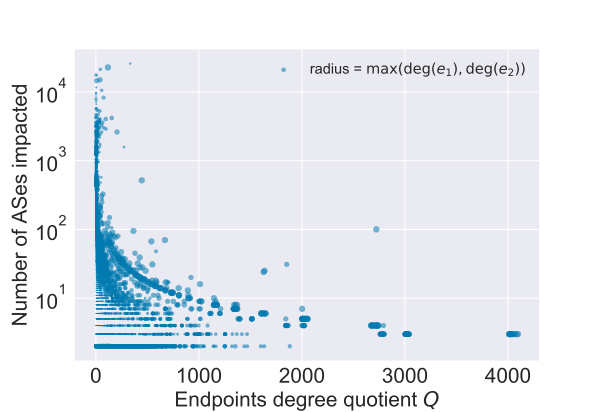
\includegraphics{figures/edg_deg_chosen.png}}
\caption{\textit{Impact} of link failures happened in March 2020}
\label{fig.impact-del-mar-2020}
}
\end{minipage}\
\end{figure}


\begin{figure}[!htb]
\begin{minipage}{0.48\textwidth}
\centering{
\resizebox{85mm}{!}{\svg{edg_deg_diff.pdf_tex}}
\caption{Difference in distributions of endpoints degrees}
\label{fig.edg-deg-diff}
}
\end{minipage}\hfill
\begin{minipage}{0.48\textwidth}
\centering{
\resizebox{85mm}{!}{\svg{hop_dist_pmf.pdf_tex}}
\caption{PMF of hop distance from broken link of impacted nodes}
\label{fig.hop-dist-pmf}
}
\end{minipage}\
\end{figure}

\section{Simulation with real link failures}
The previous simulations will now serve as the baseline to evaluate the behavior of our algorithm when considering the actual evolution of the Internet graph.

We extract the changes in the AS graph by comparing the snapshots taken in March and April by CAIDA. Since our simulator does not support live insertion/deletion of ASes, we only look at the edges. We suppose that the 42848 edges ($9.2\%$ of the total) censused in March but not in April became unavailable at some point, triggering the reaction of Internet routing algorithm.

The red line in figure \ref{fig.stretch-evo} shows the average stretch measured while progressively executing this sequence of link failures. The yellow line refers to the simulation which also considers the changes occurred in April.
It can be seen that the stretch worsens at a slower compared to the baseline. For instance, after replaying all the failures detected in March and April, the average stretch incurs a $1\%$ penalty, whereas an equal number of random deletions provokes a $6.7\%$ increase (light blue line).

\bigskip
The differences between the two simulations are due to the fact that link failures in the Internet are not randomly distributed.
Figure \ref{fig.edg-deg-diff} substantiates this claim by showing the distribution of $Q$ (the quotient between the degrees of endpoints described in section \ref{sub.impact-measurement}) over three different sets: the edges of the AS graph, those which failed during March 2020 and the 3000 random sample used in our tests above.
The shaded area highlights that links with $Q$ between 1 and 30 fail are less likely to fail, i.e. their are under-represented among the edges which failed.

This is not surprising since the edges connecting important ASes ($Q \approx 1$ and $R \gg 1$), which are more stable than the average link, fall in this category.
In fact, only $8.5\%$ of link failures involve edges incident to one of the 64 biggest ASes (by customer cone size), down from $17\%$ with randomly chosen deletions. 

\bigskip
We note that the landmarks selection strategy presented in \ref{sec.landmarks-sel} is helpful in this scenario since the topology undergoes few changes in proximity of important ASes, which are also more likely to be landmarks. Paths to those ASes, known to many other nodes, change less frequently and thus only the lower ranks of the AS hierarchy experience bunch quality deterioration. 

Further proof of this can be found in the distribution of hop-distances traveled by invalidation messages, illustrated in figure \ref{fig.hop-dist-pmf}. A third of the nodes that receive invalidation messages generated by real link failures are endpoints of one of the unstable edges (they are at hop-distance $0$), against $10\%$ with random deletions. Invalidation messages reach, on average, nodes which are only $1.2$ hops away from the failing link (down from $1.75$ with random deletions).

Even the \textit{Impact} of real link failures, depicted in figure \ref{fig.impact-del-mar-2020}, improves compared to the baseline. Its average and standard deviation, respectively of $36$ and $341$ ASes, are a third of the values obtained with random deletions.

\bigskip


%\begin{minipage}{0.48\textwidth}
%\centering{
%\resizebox{85mm}{!}{\svg{impact_3000_random.pdf_tex}}
%\caption{Impact of edges disappeared during March 2020 [TODO: edg\_deg\_chosen]}
%\label{fig.edg-deg-mar-2020}
%}
%\end{minipage}\

\chapter*{Concluding remarks}
In this project, we design a compact routing scheme for the Internet based on previous work by Thorup and Zwick. This algorithm complies with Internet-specific requirements regarding the stretch and shape of its paths estimates.
We perform simulations using the real AS graph and investigate the behavior of the scheme in the event of topology changes. 

\bigskip
We conclude that the structure of the Internet graph makes it possible to efficiently apply compact routing even in the case of a dynamic topology. The majority of edge deletions have a bearing on the state of a limited number of Autonomous Systems.

\noindent
We also show that the average communication cost for edge failures is even lower when considering the real edge failures occurring in the AS graph. 

\bigskip
One of the limitations of our approach relates to bunch quality deterioration. We believe that it can be avoided by making ASes periodically run cleanup routines, but we leave the analysis of this solution to future works.


%[we have: studied AS graph, proposed and tested reaction to edge deletion]

%[concluding remarks: periodically rerun dijkstra from other nodes]

\cleardoublepage
\phantomsection
\addcontentsline{toc}{chapter}{Bibliography}
\nocite{*}
\printbibliography

\end{document}
